\documentclass[10pt]{article}

\usepackage{pgfplots}
\newcommand{\sansserifformat}[1]{\fontfamily{cmss}{ #1}}

\title{
  Data Structure: Theoretical Approach\\ Ashraful Alam\\ Noakhali Science and Technology University\\ Information and Communication Engineering 
 }
 



\date{}

\begin{document}
\maketitle
\section{Abastract}

Run  with  accordance  with significance.  The first  if these this paper explains about the basic terminologies used  in  this  paper  in  data structure.  Better  running times will be  other constraints,  such as memory use which will  be paramount.  The most appropriate  data structures and algorithms rather than through hacking removing  a  few  statements  by  some  clever coding. Data  structures  serve  as  the  basis  for  abstract  data types (ADT). "The ADT defines the logical form  of the  data  type.  The  data  structure  implements  the physical form of the data type."Different types of data structures are suited to different kinds of applications, and some are highly specialized to specific tasks. For example,  relational  databases  commonly  use  B-tree indexes  for  data  retrieval,  while  compiler implementations  usually use  hash tables  to  look  up identifiers.




\section{Introduction}

Data  structures  serve  as  the  basis  for  abstract  data types (ADT). "The ADT defines the logical form  of the  data  type.  The  data  structure  implements  the physical form of the data type."Different types of data structures are suited to different kinds of applications, and some are highly specialized to specific tasks. For example,  relational  databases  commonly  use  B-tree indexes  for  data  retrieval,  while  compiler implementations  usually use  hash tables  to look  up identifiers. Data structures provide a means to manage large amounts of data efficiently for uses such as large databases  and  internet  indexing  services.  Usually, efficient data structures are key to designing efficient algorithms.  Some  formal  design  methods  and programming  languages  emphasize  data  structures, rather than algorithms, as the key organizing factor in software  design. 



\section{Sequential search}

The items have been placed randomly into the list.  In other words, the probability that the item we  are  looking  for  is  in  any  particular  position  is exactly the same for each position of the list.   If the item is not in the list, the only way to know it is to compare it against every item present. If there are \(n\)  items, then  the sequential  search  requires  \(n\) comparisons to discover that the item is not there. In the case  where the item is in the list,  the analysis is not  so  straightforward.  There  are  actually  three different scenarios that can occur. In the best case we will  find the  item in  the  first  place  we  look,  at the beginning  of  the  list.  We  will  need  only  one comparison. In the worst  case, we  will not  discover the  item  until  the  very  last  comparison,  the  nth comparison.

\section{Table}

\begin{tabular}{|c|c|c|}
\hline
  Algorithm & Best Case & Expected\\
  \hline
   SELECTION SHORT & O(N2) & O(N2)\\
   \hline
   MERGE SHORT & O(N2) & O(N2)\\
   \hline
   LINEAR SEARCH & O(N2) & O(N2)\\
   \hline
\end{tabular}


\section{Graphics/Images}

All images must be embedded in your document or included with your submission as individual source files. The type of graphics you include will affect the quality and size of your paper on the electronic document disc. In general, the use of vector graphics such as those produced by most presentation and drawing packages can be used without concern and is encouraged.

\begin{itemize}
\setlength\itemsep{0em}
\item Resolution: 600 dpi
\item Color Images: Bicubic Downsampling at 300dpi
\item Compression for Color Images: JPEG/Medium Quality
\item Grayscale Images: Bicubic Downsampling at 300dpi
\item Compression for Grayscale Images: JPEG/Medium Quality
\item Monochrome Images: Bicubic Downsampling at 600dpi
\item Compression for Monochrome Images: CCITT Group 4
\end{itemize}

If your paper contains many large images they will be down-sampled to reduce their size during the conversion process.  However the automated process used will not always produce the best image, and you are encouraged to perform this yourself on an image by image basis. The use of bitmapped images such as those produced when a photograph is scanned requires significant storage space and must be used with care.

\section{Main text}

Type your main text in 10-point Times, single-spaced. Do not use double-spacing. All paragraphs should be indented 1/4 inch (approximately 0.5 cm).  Be sure your text is fully justified—that is, flush left and flush right. Please do not place any additional blank lines between paragraphs. \\
\textbf{Figure and table captions} should be 9-point boldface Helvetica (or a similar sans-serif font).  Callouts should be 9-point non-boldface Helvetica. Initially capitalize only the first word of each figure caption and table title. Figures and tables must be numbered separately. For example: ``Figure 1. Database contexts'', ``Table 1. Input data''. Figure captions are to be centered below the figures. Table titles are to be centered above the tables.

% For one-column wide figures use
\begin{figure}[thb]
	% Use the relevant command to insert your figure file.
	% For example, with the graphicx package use
    \centering
	\includegraphics[\linewidth]{images/Shovo[1]-min.jpg}
	% figure caption is below the figure
	\caption{Ashraful Alam}
	\label{fig: sample-figure}       % Give a unique label
\end{figure}

\section{First-order headings}

For example, “1. Introduction”, should be Times 12-point boldface, initially capitalized, flush left, with one 12-point blank line before, and one blank line after. Use a period (“.”) after the heading number, not a colon. 

\subsection{Second-order headings}
 
As in this heading, they should be Times 11-point boldface, initially capitalized, flush left, with one blank line before, and one after. 

\subsubsection{Third-order headings. }

Third-order headings, as in this paragraph, are discouraged. However, if you must use them, use 10-point Times, boldface, initially capitalized, flush left, followed by a period and your text on the same line. 


\subsection{Math Equation}
The well known Pythagorean theorem \(x^2 + y^2 = z^2\) was 
proved to be invalid for other exponents. 
Meaning the next equation has no integer solutions:

\[ x^n + y^n = z^n \]


\subsection{Grap}
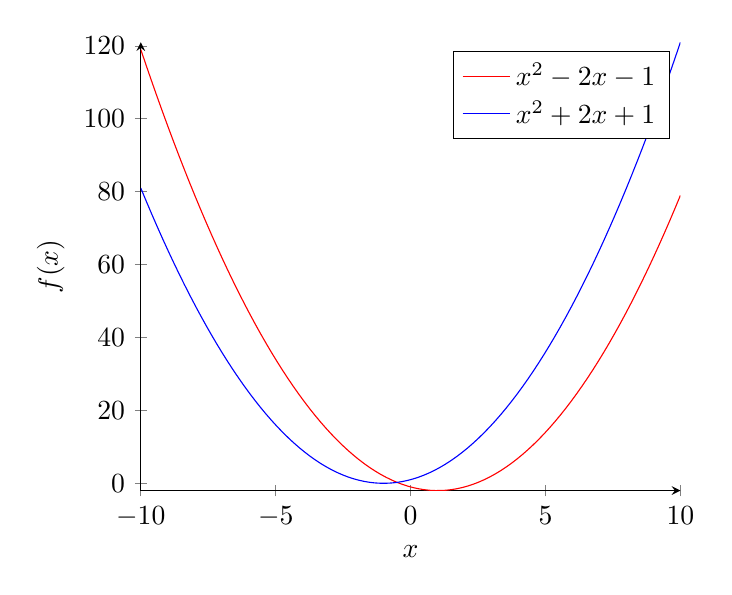
\begin{tikzpicture}
\begin{axis}[
    axis lines = left,
    xlabel = \(x\),
    ylabel = {\(f(x)\)},
]

\addplot [
    domain=-10:10, 
    samples=100, 
    color=red,
]
{x^2 - 2*x - 1};
\addlegendentry{\(x^2 - 2x - 1\)}
%Here the blue parabola is defined
\addplot [
    domain=-10:10, 
    samples=100, 
    color=blue,
    ]
    {x^2 + 2*x + 1};
\addlegendentry{\(x^2 + 2x + 1\)}

\end{axis}
\end{tikzpicture}
\section{Third-order headings. }

Third-order headings, as in this paragraph, are discouraged. However, if you must use them, use 10-point Times, boldface, initially capitalized, flush left, followed by a period and your text on the same line. 
Third-order headings, as in this paragraph, are discouraged. However, if you must use them, use 10-point Times, boldface, initially capitalized, flush left, followed by a period and your text on the same line. Third-order headings, as in this paragraph, are discouraged. However, if you must use them, use 10-point Times, boldface, initially capitalized, flush left, followed by a period and your text on the same line. Third-order headings, as in this paragraph, are discouraged. However, if you must use them, use 10-point Times, boldface, initially capitalized, flush left, followed by a period and your text on the same line. Third-order headings, as in this paragraph, are discouraged. However, if you must use them, use 10-point Times, boldface, initially capitalized, flush left, followed by a period and your text on the same line. Third-order headings, as in this paragraph, are discouraged. However, if you must use them, use 10-point Times, boldface, initially capitalized, flush left, followed by a period and your text on the same line. Third-order headings, as in this paragraph, are discouraged. However, if you must use them, use 10-point Times, boldface, initially capitalized, flush left, followed by a period and your text on the same line. Third-order headings, as in this paragraph, are discouraged. However, if you must use them, use 10-point Times, boldface, initially capitalized, flush left, followed by a period and your text on the same line. Third-order headings, as in this paragraph, are discouraged. However, if you must use them, use 10-point Times, boldface, initially capitalized, flush left, followed by a period and your text on the same line. 
\section{Fourth Order Heading}
Fourth-order headings, as in this paragraph, are discouraged. However, if you must use them, use 10-point Times, boldface, initially capitalized, flush left, followed by a period and your text on the same line. Third-order headings, as in this paragraph, are discouraged. However, if you must use them, use 10-point Times, boldface, initially capitalized, flush left, followed by a period and your text on the same line. 
Third-order headings, as in this paragraph, are discouraged. However, if you must use them, use 10-point Times, boldface, initially capitalized, flush left, followed by a period and your text on the same line. Third-order headings, as in this paragraph, are discouraged. However, if you must use them, use 10-point Times, boldface, initially capitalized, flush left, followed by a period and your text on the same line. 
\section{References} 

References and in-text citation should be in line with the format recommended by the Publication Manual of the American Psychological Association (7th edition). The style and grammar guidelines are freely available and can be found at:  \url{https://apastyle.apa.org/style-grammar-guidelines}.

List and number all bibliographical references in 9-point Times, single-spaced, and in an alphabetical order at the end of your paper. For example, \cite{Castells2010, Allen1997} and \cite{Bloomberg2018} and \cite{Allen1997}.

% if added before the last page, this command can help balancing columns
%\addtolength{\textheight}{-.2cm} 

%Bibliography 
% \bibliographystyle{apalike}
% \bibliography{sample}

\printbibliography

\end{document}
